\documentclass[hyperref={dvipdfmx,pdfpagelabels=false}]{beamer}
\title{Einführung in Matlab - Einheit 2}
\subtitle{Numerische Lineare Algebra, Programmieren}
\mode<article>
{
  \usepackage{fullpage}
  \usepackage{pgf}
  \usepackage{hyperref}
  \setjobnamebeamerversion{beamer}
}

\mode<presentation>
{
  %\usetheme{Frankfurt}
 %\usetheme{My}
  \usetheme{Madrid}
  % or ...
%\usecolortheme{seagull}
  %\setbeamercovered{transparent}
  %\setbeamercovered{dynamic}
  % or whatever (possibly just delete it)
}
\usenavigationsymbolstemplate{}
\usefonttheme{structurebold}
\usepackage{multimedia}
\usepackage{tikz}
\usepackage{fontspec,xunicode,xltxtra}
%\usepackage[scaled=.90]{helvet}
% Or whatever. Note that the encoding and the font should match. If T1
% does not look nice, try deleting the line with the fontenc.

\setbeamertemplate{footline}
{
\leavevmode
%\hbox{\begin{beamercolorbox}[wd=.5\paperwidth,ht=2.5ex,dp=1.125ex,
%leftskip=.3cm plus1fill,rightskip=.3cm]{author in head/foot}%
%    \usebeamerfont{author in head/foot}\insertshortauthor
%  \end{beamercolorbox}%
%  \begin{beamercolorbox}[wd=.5\paperwidth,ht=2.5ex,dp=1.125ex,leftskip=.3cm,
%rightskip=.3cm plus1fil]{title in head/foot}%
%    \usebeamerfont{title in head/foot}\insertshorttitle\hfill

\hfill\insertframenumber  \hspace{3pt}

%\inserttotalframenumber
%\hspace*{2ex}
%  \end{beamercolorbox}}%
  \vskip3pt%
}

%\usepackage[english]{babel}
\usepackage[ngerman]{babel}
\selectlanguage{ngerman}

%
% math/symbols
%
\usepackage{amssymb}
\usepackage{amsthm}
% \usepackage{latexsym}
\usepackage{amsmath}
%\usepackage{listings}
\usepackage[framed]{mcode}
%\usepackage{mcode}

\usepackage{mydef}
\usepackage{cmap} % you can search in the pdf for umlauts and ligatures
%\usepackage{colonequals} %corrects the definition-symbols \colonequals (besides others)
\title{Einführung in Matlab}
%
%\subtitle{Disputation} % (optional)

\author{Jochen Schulz}
% - Use the \inst{?} command only if the authors have different
%   affiliation.

\institute{Georg-August Universit\"at G\"ottingen \pgfimage[height=0.5cm]{../figures/unilogo3}}
% - Use the \inst command only if there are several affiliations.
% - Keep it simple, no one is interested in your street address.

\date{\today}

\subject{Einführung in Matlab}
% This is only inserted into the PDF information catalog. Can be left
% out. 



% If you have a file called "university-logo-filename.xxx", where xxx
% is a graphic format that can be processed by latex or pdflatex,
% resp., then you can add a logo as follows:

%\logo{\pgfimage[height=0.5cm]{figures/unilogo3}}


% Delete this, if you do not want the table of contents to pop up at
% the beginning of each subsection:
% \AtBeginSubsection[]
% {
%   \begin{frame}<beamer>
%     \frametitle{Aufbau}
%     \tableofcontents[currentsection,currentsubsection]
%   \end{frame}
% }

\AtBeginSection[]
{
  \begin{frame}<beamer>
    \frametitle{Aufbau}
    \tableofcontents[currentsection,currentsubsection]
  \end{frame}
}


\begin{document}



\maketitle

\section{Numerische Lineare Algebra}

\subsection{Normen}
% 
% Slide
%
\begin{frame}[fragile]\frametitle{Vektornorm}
Die $p$-Norm eines Vektors $x=(x_1, {} \dots , x_n)$
\[ \|x \|_p := \left( \sum_{i=1}^n  |x_i|^p \right)^{1/p} \] 
(definiert für $p\geq 1$).
\begin{itemize}
\item in MATLAB: \mcode{norm(x,p)} (Default: $p=2$) 
\item $p=\infty$ entspricht der Maximum-Norm 
\[  \|x \|_\infty = \max_{i=1, \dots n} |x_i|. \]
\end{itemize}
\end{frame}
% 
% Slide
%
\begin{frame}[fragile]\frametitle{Matrixnorm}
Seien  $A\in \mathbb{C}^{n \times m}$ und
$p \geq 1$. Die
{\it Matrixnorm} ist definiert durch
\[ \| A \|_p = \sup_{x\in \mathbb{C}^m \setminus \{ 0 \}} \frac{\|Ax
  \|_p}{\| x \|_p}. \]
\begin{itemize}
\item In MATLAB: \mcode{norm(A,p)} (Default $p=2$).
\item $p=\infty$ kann charakterisiert werden durch
\[ \|A\|_\infty = \max_{1 \leq j \leq m} \sum_{i=1}^n |a_{ij}|, \quad
\mbox{Zeilensummennorm.} \]
\end{itemize} 
\end{frame}
% 
% Slide
%
\begin{frame}[fragile]\frametitle{Kondition}
Kondition einer quadratischen Matrix $A$: 
{ \[ \cond_p(A):=\|A\|_p\|A^{-1}\|_p. \] }
\vspace*{-0.8cm}
\begin{itemize}
\item In MATLAB: 
  \mcode{cond(A,p)} (Default $p=2$) 
\item Es gilt $\cond_p(A)\geq 1$.
\item Die Kondition mißt die Empfindlichkeit der Lösung $x$ von $Ax=b$
  gegenüber  Störungen
  von $A$ und $b$.
\item Ist $\cond_p(A) >> 1$, so ist die Matrix beinahe singulär. Die Matrix ist {\it schlecht konditioniert}.
\end{itemize}
\end{frame}
% 
% Slide
%
\begin{frame}[fragile]\frametitle{Beispiele}
\begin{itemize}
\item Vektornormen für $x=(1/100) (1, 2, \dots, 100)$
\begin{lstlisting}
>> x = (1:100)/100; [norm(x,1) norm(x,2) norm(x,inf)]
ans =   50.5000    5.8168    1.0000
\end{lstlisting}
\item Matrixnorm für die Hilbert-Matrix $H=(\frac{1}{i+j-1})_{ij}$
\begin{lstlisting}
>> H = hilb(10); [norm(H,1) norm(H,2) norm(H,inf)]
ans =    2.9290    1.7519    2.9290
\end{lstlisting}
\item Kondition der Hilbert-Matrix
\begin{lstlisting}
>> H = hilb(10); [cond(H,1) cond(H,2) cond(H,inf)]
ans =
   1.0e+13 *
    3.5354    1.6025    3.5354
\end{lstlisting}
\end{itemize}
\end{frame}

\subsection{Lösen linearer Gleichungssyteme}
% 
% Slide 
%
\begin{frame}[fragile]\frametitle{Lineare Gleichungssysteme}
Seien $A \in \mathbb{C}^{n\times n}$ und $b \in \mathbb{C}^n$. Das
lineare Gleichungssystem 
{ \[ A x=b \]}
wird in MATLAB gelöst durch  \mcode{ x=A\\b}.\\

\begin{lstlisting}
>> x = ones(5,1); H = hilb(5); b = H*x; y = (H\b)'
y =
    1.0000    1.0000    1.0000    1.0000    1.0000
\end{lstlisting}

\alert{Warnung:} Benutze nie
\mcode{x=inv(A)*b}, da das Berechnen von $A^{-1}$ sehr aufwendig sein kann.
\end{frame}
% 
% Slide 
%
\begin{frame}[fragile]\frametitle{LU-Zerlegung}
{\centering  Was bedeutet \mcode{A\\b}?}\\[0.5cm]

MATLAB berechnet die LU-Zerlegung von $A$ (Gaussverfahren):
\begin{itemize}
 \item obere Dreiecksmatrix $U$
 \item untere Dreiecksmatrix $L$ mit Einsen auf der Diagonalen
\end{itemize}
so dass $PA=LU$ gilt ($P$ Permutationsmatrix).

Dann wird das LGS durch Rückwärts- und Vorwärtseinsetzen gelöst
($Lz = Pb$, $Ux = z$)

\begin{lstlisting}
>> [L,U,P]=lu(hilb(5)); norm(P*hilb(5)-L*U)
ans =  2.7756e-17
\end{lstlisting}
\end{frame}
% 
% Slide 
%
\begin{frame}[fragile]\frametitle{Inverse,  Determinante}
\begin{itemize}
\item Berechnung der Inversen
\begin{columns}[onlytextwidth]
\column{0.45\textwidth}
\begin{lstlisting}
>> A=pascal(3)
A =
     1     1     1
     1     2     3
     1     3     6
\end{lstlisting}
\column{0.45\textwidth}
\begin{lstlisting}
>> X=inv(A)
X =
     3    -3     1
    -3     5    -2
     1    -2     1
\end{lstlisting}
\end{columns}
\item Berechnung der Determinante
\begin{lstlisting}
>> det(A)
ans = 1
\end{lstlisting}
\end{itemize}
\end{frame}
% 
% Slide 
%
\begin{frame}[fragile]\frametitle{Pseudoinverse}
\begin{block}{(Moore-Penrose) Pseudoinverse}
Sei $A$ singulär, Bestimme $X$ so dass 
\[ A X A=A,  X A X =X,  (X A)^* =X A,  (A X )^* = A X \]
\end{block}
\begin{lstlisting}
>> pinv(ones(3,3))
ans =
    0.1111    0.1111    0.1111
    0.1111    0.1111    0.1111
    0.1111    0.1111    0.1111
\end{lstlisting}
\end{frame}

\subsection{Anwendung: Zwei-Punkt-Randwert-Aufgabe}
%
% Slide
%
\begin{frame}[fragile]\frametitle{Zwei-Punkt-Randwert-Aufgabe}

Suche eine Funktion 
\begin{equation*}
u:[0,1] \quad \rightarrow \quad \mathbb{R}, 
\end{equation*}
so dass 
\begin{eqnarray*}
-u''(x) & = & e^x, \quad x \in (0,1)\\
u(0) & = & u(1) =0
\end{eqnarray*}
\alert{Problem:} Es kann i.A. keine geschlossene
Lösungsdarstellung angegeben werden. \\ %Wieso ?

\alert{Ausweg:} Approximation der Lösung. 
\end{frame}
%
% Slide: 
%
\begin{frame}[fragile]\frametitle{Finite Differenzen Verfahren}

Diskretisierung: $0=x_0 < \dots < x_{n}=1$ mit $x_i=\frac{i}{n}$\\

Differenzenquotient: 
\[ u''(x_i) \sim \frac{u(x_{i-1}) - 2 u(x_i) + u(x_{i+1})}{ 
  h^2}, \quad h:=\frac{1}{n} \]

Einsetzen in $-u''(x)=e^x$ ergibt 
\[ -u(x_{i-1}) + 2 u(x_i) - u(x_{i+1}) =  h^2 e^{x_i}, \quad
i=1,\dots ,n-1 \] 
Randbedingungen $\Rightarrow $ $u(x_0)=u(x_n)=0$.\\

$\Rightarrow$ Lineares Gleichungssystem für 
$u(x_1), \dots ,u(x_{n-1})$.
\end{frame}

%
% Slide: 
%
\begin{frame}[fragile]\frametitle{Diskretes Problem}

Setze $z=(z_1,\dots ,z_{n-1})^t=(u(x_1), \dots ,u(x_{n-1}))^t$. \\

Löse das Gleichungssystem  $Az=F$  mit 
\[ A:= 
\left( \begin{array} {ccccccc}
 2 & -1 &  & &   0 \\
-1 & 2  & -1 &    & \\ 
   & \ddots & \ddots & \ddots   &\\
   & &  -1 & 2  & -1  \\ 
0 &  &    & -1 & 2 \\
\end{array} \right), \  F:=
h^2 \left( \begin{array}{c} e^\frac{1}{n}\\   \vdots \\ e^\frac{n-1}{n}
\end{array} \right) .
\] 
\end{frame}
%
% Slide: 
%
\begin{frame}[fragile]\frametitle{Lösung für $n=21$}
\begin{itemize}
\item Zerlegung des Intervalls $[0,1]$
\begin{lstlisting}
x = 0:(1/21):1
\end{lstlisting}
\item Eleminieren der Randpunkte
\begin{lstlisting}
x_i = x(2:21)
\end{lstlisting}
\item Erzeugen der Matrix $A$ (Übungsaufgabe)
\end{itemize}
\end{frame}
%
% Slide: 
%
\begin{frame}[fragile]\frametitle{Lösung für $n=21$}
\begin{itemize}
\item Berechnen der rechten Seite:
\begin{lstlisting}
F = (1/21)^2*transpose(exp(x_i));
\end{lstlisting}
\item Lösen des linearen Gls.\\
\begin{lstlisting}
z_i = A\F;
\end{lstlisting}
\item Zufügen der Werte am Rand
\begin{lstlisting}
>> z = [0; z_i;0];
\end{lstlisting}
\end{itemize}
\end{frame}
%
% Slide: 
%
\begin{frame}[fragile]\frametitle{Lösung für $n=21$}
\begin{columns}[c]
\column{0.48\textwidth}
\begin{lstlisting}[basicstyle=\tiny]
plot(x,z,'r*','MarkerSize',8)
\end{lstlisting}
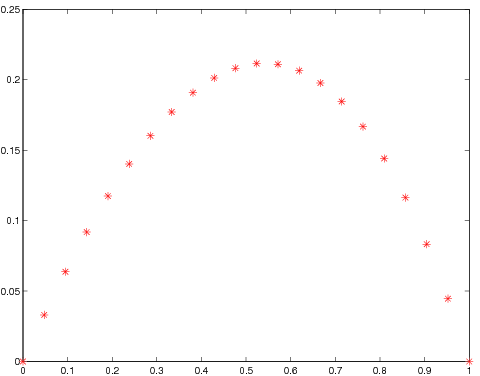
\includegraphics[width=\textwidth]{figures/bild1_27_10}

\column{0.48\textwidth}
\begin{lstlisting}[basicstyle=\tiny]
plot(x,z,'r*-','LineWidth',3,'MarkerSize',8)
\end{lstlisting}%
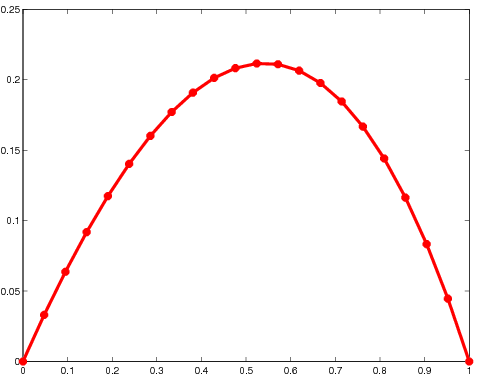
\includegraphics[width=\textwidth]{figures/bild2_27_10}
\end{columns}
\end{frame}


\subsection{Bestimmung von Eigenwerten}
% 
% Slide 
%
\begin{frame}[fragile]\frametitle{Eigenwerte}
\begin{block}{Eigenwert}
Sei $A \in \mathbb{C}^{n \times n}$. $\lambda \in \mathbb{C}$ ist
Eigenwert von $A$, falls ein Vektor $x \in \mathbb{C}^n$ ungleich $0$ existiert, so
dass  $Ax = \lambda x$ gilt. $x$ heißt Eigenvektor.  
\end{block}

\begin{itemize}
\item {}\mcode{x=eig(A)}\\ berechnet die Eigenwerte von $A$ und schreibt
  sie in den Vektor $x$.
\item
  {}\mcode{[V,D]=eig(A)}\\
  $D$ ist eine Diagonalmatrix mit den Eigenwerten auf der
  Diagonalen. Die Spalten von $V$ bilden die zugehörigen Eigenvektoren. 
\end{itemize}
\end{frame}
% 
% Slide 
%
\begin{frame}[fragile]\frametitle{Weitere Zerlegungen}
\begin{itemize}
\item \alert{QR-Zerlegung}: \mcode{[Q,R]=qr(A)}\\
  $m \times n$- Matrix $A$ eine Zerlegung { $A=QR$} erzeugt,
  ($Q$ eine unitäre $m \times m$-Matrix, $R$ eine obere $m \times n$ Dreiecksmatrix).
%Die QR-Zerlegung spielt in vielen Verfahren der numerischen Mathematik  eine wichtige Rolle, 
%beispielsweise um eine orthogonale oder unitäre Basis zu bestimmen oder um lineare Ausgleichsprobleme 
%zu behandeln. 
%QR-Algorithmus zur Berechnung aller Eigenwerte einer Matrix.
\item \alert{Singulärwertzerlegung}: \mcode{[U,S,V]=svd(A)}\\
  { $A=U \Sigma V^*$}. 
  ($\Sigma \subset \mathbb{C}^{m \times n}$ eine Diagonalmatrix \\
  $U \subset \mathbb{C}^{m \times m}$, $V \subset  \mathbb{C}^{n \times n}$ unitäre Matrizen). 
%Dieses Verfahren wird insbesondere in der numerischen Mathematik verwendet. Dort lassen sich beispielsweise quasisinguläre 
%lineare Gleichungssysteme im Rahmen rechentechnischer Genauigkeiten passabel lösen.
%In der Statistik ist die SVD der rechnerische Kern der Hauptkomponentenanalyse, dort auch Karhunen-Loève-Transformation genannt.
%Einige moderne Bildkompressionsverfahren beruhen auf einem Algorithmus, der das Bild (=Matrix aus Farbwerten) in eine SVD überführt 
%und anschließend nur die stark von null verschieden Elemente der Matrix Σ berücksichtigt und dann die zur Rückgewinnung der Matrix 
%erforderlichen Vektoren sowie die verbliebenen Diagonalelemente speichert. Besonders effektiv ist diese Kompression bei 
%bestimmten rechteckigen Mustern und natürlich, je größer (und je quadratischer) das Bild ist. Dies ist eine mögliche Anwendung 
%von Modellreduktion. Das Weglassen von kleinen Singulärwerten ist ein verlustbehaftetes Modellreduktionsverfahren.

\item \alert{Cholesky-Zerlegung}: \mcode{R=chol(A)}\\
  { $A=R^*R$} zu einer hermiteschen, positiv definiten Matrix
  $A$ ($R$ ist eine obere Dreiecksmatrix mit reellen, positiven
  Diagonalelementen). 
\end{itemize}
%Eine Matrix A heißt hermitesch (nach Charles Hermite) oder selbstadjungiert genau dann, wenn sie gleich ihrer 
%(hermitesch) Adjungierten A * , also gleich der transponierten und komplex konjugierten Matrix ist. D. h.

%positiv definit, 	falls x^T Ax > 0

%Die Cholesky-Zerlegung kann auch zur Gewinnung eines Vorkonditionierungsverfahrens für lineare Gleichungssysteme mit 
%positiv definiter Matrix benutzt werden; zu diesem Zweck gibt es speziell die Variante der unvollständigen Cholesky-Zerlegung 
%sowie der modifizierten unvollständigen Cholesky-Zerlegung.
% determinante
% test ob es eine positiv definite matrix ist
\end{frame}
% 
% Slide 
%
\begin{frame}[fragile]\frametitle{Bemerkungen}
\begin{itemize}
\item LGS können auch mit Hilfe iterativer Verfahren gelöst werden,
  z.B. \mcode{gmres}, \mcode{pcg}, \mcode{bicgstab}.
\item $A\in \mathbb{C}^{n \times m}$, $n \neq m$ bei \mcode{A\\b}:
\begin{itemize}
\item $n>m$ (überbestimmter Fall): Least-Square Lösung, d.h. der Ausdruck
  \mcode{norm(A*x-b)} wird minimiert. 
\item $n<m$ (unterbestimmter Fall): Grundlösung. 
\end{itemize}
\end{itemize}
\end{frame}

\section{Programmieren - Fixpunktiteration}
%\item Aufgaben
 
%
% Slide
%
\begin{frame}[fragile]\frametitle{Gültigkeitsbereich von Variablen}
\begin{itemize}
\item \alert{Variablen in Skript-Files} benutzen den globalen Workspace,
  d.h. bereits vorhandene Variablen können direkt benutzt oder
  überschrieben werden. Sie sind gültig bis sie explizit gelöscht
  werden.
\item \alert{Variablen in Function-Files} sind nur innerhalb der
  Funktion definiert und werden bei Verlassen der Funktion
  gelöscht. Variablen des globalen Workspace können nicht benutzt
  werden. 
\end{itemize}
\end{frame}

\subsection{Schleifen}
%
% - Folie
%
\begin{frame}[fragile]\frametitle{Fixpunkt}
Suche ein $x_f \in \mathbb{R}$ so dass
\[ x_f = \cos (x_f ) \]
\begin{center}
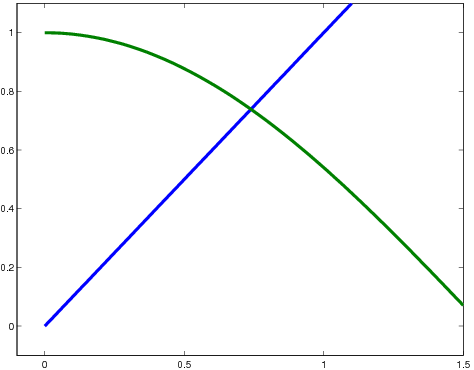
\includegraphics[height=5cm]{figures/fixpunkt}
\end{center}
\end{frame}
%
% - Folie
%
\begin{frame}[fragile]\frametitle{Fixpunkt-Iteration}
Fixpunkt-Iteration 
\[ x_{k+1}=cos(x_k) \]
bei geeignetem Startwert $x_0$.  \\
\centering{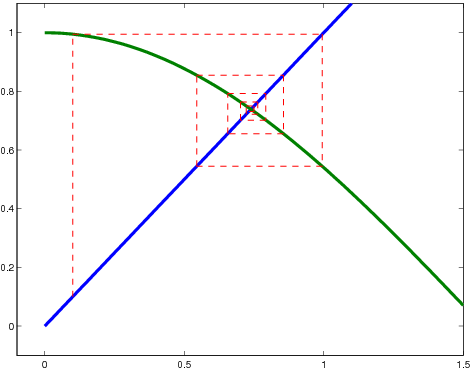
\includegraphics[height=5cm]{figures/fixpunkt1}}\\
(Funktioniert wenn die Abbildung kontrahierend ist)
\end{frame}

%
% - Folie
%
\begin{frame}[fragile]\frametitle{Implementierung}
\begin{lstlisting}
% Plot 1
x = linspace(0,1.5,50);
y = cos(x);
plot(x,x,x,y,'LineWidth',3),
axis([-0.1 1.5 -0.1 1.1]);
hold on;
pause; % stoppt bis eine Taste gedrückt wird
z(1) = 0.1; % Anfangswert
it_max = 10; % Iterationsschritte 
for i = 1:it_max
    z(i+1) = cos(z(i));
    plot([z(i) z(i)], [z(i) z(i+1)],'r--','LineWidth',1);
    pause;
    plot([z(i) z(i+1)],[z(i+1) z(i+1)],'r--','LineWidth',1);
    hold on;
    pause; % stoppt bis eine Taste gedrückt wird
end;
\end{lstlisting}
\end{frame}
%
% - Folie
%
\begin{frame}[fragile]\frametitle{Einige Grafikbefehle}
\begin{itemize}
\item Durch \alert{ \mcode{figure}} wird ein Grafik-Fenster gestartet.
\item Mittels \alert{ \mcode{hold on}} werden alle Grafiken in einem Fenster
  \"ubereinander gezeichnet. 
\item Im Standardmodus wird bei jedem Grafikbefehl die bestehende Grafik
  gel\"oscht und durch die neue Grafik ersetzt.
\item Mittels \alert{ \mcode{hold off}} wird zur\"uck in den Standardmodus
  gewechselt.  
\end{itemize}
\end{frame}
%
% - Folie
%
\begin{frame}[fragile]\frametitle{for - Schleife}
\begin{lstlisting}
for <variable> = <Ausdruck>
  <Befehle>
end
\end{lstlisting}
\alert{Bemerkungen:} 
\begin{itemize}
\item Der Ausdruck ist normalerweise von der Form
\mcode{i:s:j}. 
\item Die {\it Befehle} werden eingerückt. 
\item auch weitere Schleifen-Konstrukte wie \mcode{while} und \mcode{switch} sind verfügbar.
\end{itemize}
\end{frame}
%
% - Folie
%
\begin{frame}[fragile]\frametitle{Beispiele}
\begin{itemize}
\item Berechne $\sum_{i=1}^{1000} \frac{1}{i}$
\begin{lstlisting}
>> sum=0; for j=1:1000, sum=sum+1/j; end, sum
sum =  7.4855
\end{lstlisting}
\item Berechnen dreier Werte
\begin{lstlisting}
>> for x=[pi/6 pi/4 pi/3], sin(x), end
ans =    0.5000
ans =    0.7071
ans =    0.8660
\end{lstlisting}
\item Matrix als {\it Ausdruck}
\begin{lstlisting}
>> for x=eye(3),  x' ,end
ans =     1     0     0
ans =     0     1     0
ans =     0     0     1
\end{lstlisting}
\end{itemize}
\end{frame}
\begin{frame}[fragile]\frametitle{Vandermonde-Matrix }
Berechne zu einem gegebenen Vektor
  $x=(x_1, \dots ,x_n)$ die Vandermonde-Matrix
{ \[ V:= \left(\begin{array}{ccccc} 
1 & x_1 & x_1^2 & \hdots & x_1^{n-1}\\
1 & x_2 & x_2^2 & \hdots & x_2^{n-1}\\
\vdots & \vdots & \vdots & \vdots & \vdots\\
1 & x_n & x_n^2 & \hdots & x_n^{n-1}\\
\end{array} \right).  \]}
\end{frame}
%
%
%
\begin{frame}[fragile]\frametitle{Implementierung II}
\lstinputlisting{vandermonde2.m}
\end{frame}

\subsection{Bedingungen}
%
%
%
\begin{frame}[fragile]\frametitle{Quadratische Gleichung}
\alert{ \[  \left\{ \begin{array}{l} \mbox{Suche }  x \in \mathbb{R},
 \mbox{ so dass } \\
 x^2+px +q =0  \end{array} \right. \]}
Fallunterscheidung für $d:=\frac{p^2}{4} -q$:
\begin{description}
\item [Fall a)]: \alert{ $d>0$} \quad 2 Lösungen: $x=-\frac{p}{2} \pm \sqrt{d}$ \\
\item [Fall b)]: \alert{ $d=0$} \quad 1 Lösung: $x=-\frac{p}{2}$\\
\item [Fall c)]: \alert{ $d<0$} \quad keine Lösung
\end{description}
\end{frame} 
%
%
%
\begin{frame}[fragile]\frametitle{Implementierung}
\begin{lstlisting}
function [anz_loesungen, loesungen]=quad_gl(p,q)
%----------------------------------------------------
% quad_gl berechnet die Loesungen der quadratischen   
%         Gleichung x^2 + px + q =0
%           INPUT:   Skalare   p
%                              q
%                 
%           OUTPUT: anz_loesungen   Anzahl der Loesungen
%                   loesungen       Vektor der Loesungen
%
%  Gerd Rapin      8.11.2003
%------------------------------------------------------
d=p^2/4-q; % Diskriminante


\end{lstlisting}
\end{frame}
%
%
%
\begin{frame}[fragile]\frametitle{Implementierung II}
\begin{lstlisting}
% 2 Loesungen
if d>0 
    anz_loesungen=2;
    loesungen=[-p/2-sqrt(d) -p/2+sqrt(d)];
end

% 1 Loesung
if d==0 
    anz_loesungen=1;
    loesungen=[-p/2];
end

% 0 Loesungen
if d<0 
    anz_loesungen=0;
    loesungen=[];
end
\end{lstlisting}
\end{frame}

%
%
%
\begin{frame}[fragile]\frametitle{Logische Operationen}
\begin{itemize}
\item Es gibt in MATLAB logische Variablen. Der Datentyp ist {\it
  logical}. 
\item Variablen dieses Typs sind entweder \mcode{TRUE} (1) oder
  \mcode{FALSE} (0).
\item Numerische Werte ungleich $0$ werden als \mcode{TRUE} gewertet.
\end{itemize}
\begin{lstlisting}
>> a = (1<2)
a = 1
>> b = ([ 1 2 3 ] < [ 2 2 2 ])
b =   1     0     0
>> whos
  Name Size Bytes  Class
  a     1x1  1  logical array
  b     1x3  3  logical array
\end{lstlisting}
\end{frame}
%
%
%
\begin{frame}[fragile]\frametitle{Vergleichs-Operatoren}
\begin{lstlisting} 
>> a=[1 1 1], b=[0 1 2] 
\end{lstlisting}
\begin{center}
\begin{tabular}{cll}
Operation & Bedeutung & Ergebnis\\
\hline
\mcode{a == b} & gleich &   \mcode{0     1     0}\\
\mcode{a \~= b} & ungleich & \mcode{1     0     1}\\
\mcode{a < b} & kleiner & \mcode{0     0     1}\\
\mcode{a > b} & größer & \mcode{1     0     0}\\
\mcode{a <= b} & kleiner oder gleich & \mcode{0     1     1}\\
\mcode{a >= b} & größer oder gleich & \mcode{1     1     0}\\
\end{tabular}
\end{center}
\alert{Bem:} \alert{ 1 = wahre Aussage, 0 = falsche Aussage}\\
\alert{Bem:} Komponentenweise Vergleiche sind auch für Matrizen
gleicher Größe möglich! 
\end{frame}
%
%
%
\begin{frame}[fragile]\frametitle{Logische Operatoren}
\begin{center}
\begin{tabular}{|c|l||c|l|}
\hline
\mcode{\&} & logisches und & \mcode{\~} & logisches nicht \\
\mcode{|} & logisches oder & \mcode{xor} & exklusives oder\\
\hline
\end{tabular}
\end{center}
Beispiele:\\
\begin{lstlisting} 
>>  x=[-1 1 1]; y=[1 2 -3];
\end{lstlisting}
\vspace*{0.5cm}
\begin{minipage}{5cm}
\begin{lstlisting}
>> (x>0) & (y>0)
ans =
     0     1     0
\end{lstlisting}
\vspace*{0.5cm}
\begin{lstlisting}
>> (x>0) | (y>0)
ans =
     1     1     1
\end{lstlisting}
\end{minipage} \hfill
\begin{minipage}{5cm}
\begin{lstlisting}
>> ~( (x>0) & (y>0))
ans =
     1     0     1
\end{lstlisting}
\vspace*{0.5cm}
\begin{lstlisting}
>> xor(x>0,y>0)
ans =
     1     0     1
\end{lstlisting}
\end{minipage}
\end{frame}
%
%
%
\begin{frame}[fragile]\frametitle{Bedingung}
\begin{columns}[t,onlytextwidth]
 \column{0.45\textwidth}
Einfache Bedingung
\begin{lstlisting}
if  <Ausdruck>
   <Befehle>
end
\end{lstlisting}
 \column{0.45\textwidth}
Bed. mit Alternative
\begin{lstlisting}
if  <Ausdruck>
   <Befehle>
else
   <Befehle>
end
\end{lstlisting}
\end{columns}

Die Befehle zwischen \mcode{if} und \mcode{end} werden ausgeführt, wenn
der \textit{Ausdruck} wahr (\mcode{TRUE}) ist. 
Andernfalls werden (soweit vorhanden) die
Befehle zwischen \mcode{else} und \mcode{end} ausgeführt.

\textit{Ausdruck} ist wahr, wenn   alle Einträge von \textit{Ausdruck} ungleich $0$ sind.
\end{frame}
%
%
%
\begin{frame}[fragile]\frametitle{While-Schleifen}
\begin{lstlisting}
while <Ausdruck>
   <Befehle>
end
\end{lstlisting}
Die Befehle werden wiederholt,  so lange die Bedingung {\it Ausdruck}
wahr ist.  {\it Ausdruck} ist wahr, wenn   alle Einträge von {\it
  Ausdruck} ungleich $0$ sind. \\[1cm] 

\textbf{Beispiel:} Berechne \alert{ $\sum_{i=1}^{1000} \frac{1}{i}$}.
\begin{lstlisting}
n = 1000; sum = 0; i = 1; 
while (i <= n) 
  sum = sum+(1/i); 
  i = i+1;  
end
sum
\end{lstlisting}

\end{frame}
%
%
%
\begin{frame}[fragile]\frametitle{Größter gemeins. Teiler (ggT)}
Berechnung des ggT von natürlichen Zahlen $a$ und $b$ mit Hilfe des
euklidischen Algorithmus\\[1cm]

\alert{Idee:} Es gilt \alert{ $ggT(a,b)=ggT(a,b-a)$} für $a<b$.\\[1cm]

\alert{Algorithmus:} \\
Wiederhole,  bis $a=b$
\begin{itemize}
\item Ist $a>b$, so $a=a-b$.
\item Ist $a<b$, so $b=b-a$ 
\end{itemize}
\end{frame}

\begin{frame}[fragile]\frametitle{Implementierung}
\lstinputlisting{ggt.m}
\end{frame}
%
%
%
\begin{frame}[fragile]\frametitle{\textit{break}}
\begin{itemize}
\item  Der Befehl \mcode{break} verläßt die \mcode{while} oder
  \mcode{for}-Schleife.
\begin{matlabin}
x=1;
while 1
  xmin=x;
  x=x/2;
  if x==0
    break
  end
end
xmin
\end{matlabin}
\begin{matlab}
xmin = 4.9407e-324
\end{matlab} 

\end{itemize}
\end{frame}

\begin{frame}[fragile]\frametitle{\textit{continue}}
\begin{itemize}
 \item  Durch \mcode{continue} springt man sofort in die
  nächste Iteration der Schleife, ohne die restlichen Befehle zu
  durchlaufen.
\begin{matlabin}
for i=1:10
  if i<5
    continue
  end
  x(i)=i;
end
x
\end{matlabin}
\begin{matlab}
x =  0  0  0  0  5  6  7  8  9  10
\end{matlab}
 
\end{itemize}
\end{frame}


\subsection{Rekursionen}
%
% Slide
% 
\begin{frame}[fragile]\frametitle{Rekursive Funktionen}
Rekursive Funktionen sind Funktionen, die sich selbst aufrufen.\\
Bei jedem Aufruf wird ein neuer lokaler Workspace erzeugt.\\[1cm]

\textbf{Beispiel:} Fakult"at: $n!=\fak(n)$\\
\begin{eqnarray*}
 n!& = & n(n-1)!=n \fak(n-1)\\
& = & n(n-1)\fak(n-2)\\
& = & \cdots= n(n-1)\cdots 1 
\end{eqnarray*}
\end{frame}
%
% Slide
%
\begin{frame}[fragile]\frametitle{Fakult"at - rekursiv}
\lstinputlisting{fak.m}
\end{frame}
%
% Slide
%
\begin{frame}[fragile]\frametitle{Fakult"at - direkt}
\lstinputlisting{fak_it.m}
\end{frame}
%
% Slide
%
\begin{frame}[fragile]\frametitle{Fakult"at - Zeitvergleich}
\lstinputlisting{fak_vergleich.m}
\end{frame}
%
% Slide
%
\begin{frame}[fragile]\frametitle{rekursive Implementierung GGT}
\lstinputlisting{ggt_rekursiv.m}
\end{frame}
%
% Slide
% 
\begin{frame}[fragile]\frametitle{Sierpinski Dreieck}
\begin{itemize}
\item Wir beginnen mit einem Dreieck mit Eckpunkten $P_a$, $P_b$ und $P_c$. 
\item Wir entfernen daraus das Dreieck, das durch die Mittelpunkte der
  Kanten entsteht.
\item Die verbliebenden drei Dreiecke werden der gleichen Prozedur
  unterzogen.
\item Diesen Prozess können wir rekursiv wiederholen.
\item Das Ergebnis ist das Sierpinski Dreieck.
\end{itemize}
\end{frame}
%
% Slide
% 
\begin{frame}[fragile]\frametitle{Sierpinski Dreieck}
\begin{minipage}{5cm}
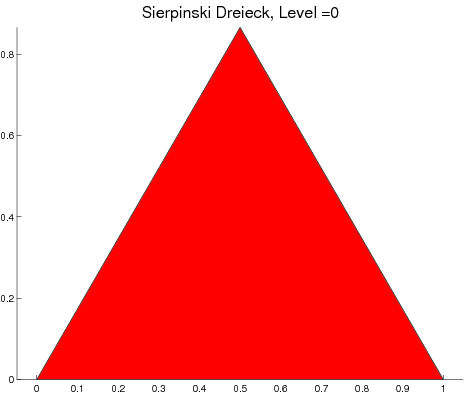
\includegraphics[height=4cm]{figures/sierpinski_0}
\end{minipage} \hfill
\begin{minipage}{5cm}
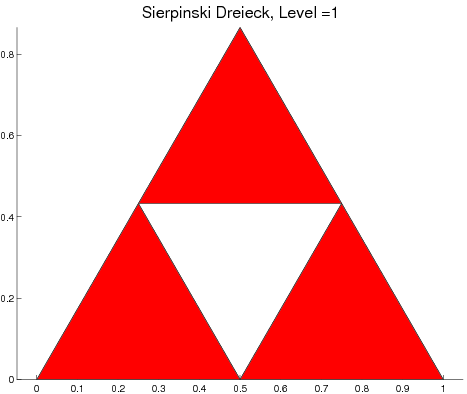
\includegraphics[height=4cm]{figures/sierpinski_1}
\end{minipage}\\ 
\begin{minipage}{5cm}
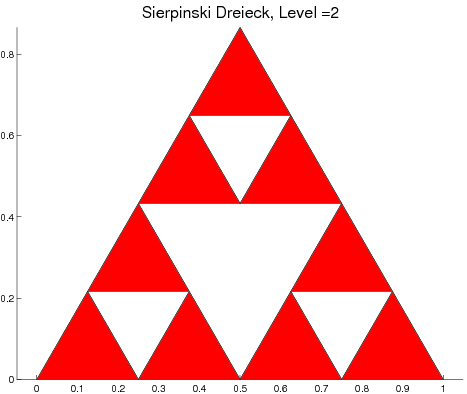
\includegraphics[height=4cm]{figures/sierpinski_2}
\end{minipage} \hfill
\begin{minipage}{5cm}
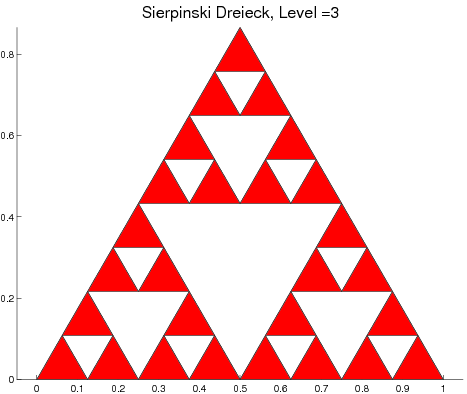
\includegraphics[height=4cm]{figures/sierpinski_3}
\end{minipage} \\
\end{frame}
%
% Slide
%
\begin{frame}[fragile]\frametitle{Implementierung}
\lstinputlisting{sierpinski_plot.m}
\end{frame}
%
% Slide
%
\begin{frame}[fragile]\frametitle{Implementierung}
\lstinputlisting{sierpinski.m}
\end{frame}
% 
% Slide
% 
\begin{frame}[fragile]\frametitle{Zeichnen von Polygonen}

Ein Polygon sei durch die Eckpunkte $(x_i,y_i)_{i=1}^n$ gegeben. Dann
kann er in MATLAB durch den Befehl
\begin{lstlisting}
fill(x,y,char)
\end{lstlisting}
dargestellt werden. \mcode{char} gibt die Farbe des Polygons an, z.B. rot
wäre 'r'.
\end{frame}

\subsection{Allgemeines}
%
% Slide
%
\begin{frame}[fragile]\frametitle{Warnung}
\begin{center}
\alert{ Wiederholte Anwendung von Script-Files kann zu Fehlern führen!}\\[0.5cm]
\end{center}
\begin{columns}[t]
 \column{0.4\textwidth}
\alert{Programm}
\begin{lstlisting}[basicstyle=\scriptsize]
% plotte_sin.m

disp(['Plot der Sinus'...
  'Funktion auf [0,10]']);
n = input(['Plot an '...
   'wievielen Punkten?']);
x = linspace(0,10,n);
for i=1:n
y(i) = sin(x(i));
end; 
plot(x,y);
\end{lstlisting}
\column{0.5\textwidth}
\alert{ Aufruf}
\begin{lstlisting}[basicstyle=\scriptsize]
>> plotte_sin
Plot der Sinus Funktion auf [0,10]
Plot an wievielen Punkten?20
>> plotte_sin
Plot der Sinus Funktion auf [0,10]
Plot an wievielen Punkten?10
??? Error using ==> plot
Vectors must be the same lengths.

Error in ==> plotte_sin.m
On line 9  ==> plot(x,y);
\end{lstlisting}
\end{columns}
\end{frame}
%
% Slide
%
\begin{frame}[fragile]\frametitle{globale Variablen}
Mittels des Befehls \alert{ \mcode{global}} können Variablen des
globalen Workspace auch für Funktionen manipulierbar gemacht werden.
\bigskip
\begin{columns}[t]
 \column{0.45\textwidth}
\alert{ Funktion}
\begin{lstlisting}
function f=myfun(x)
% myfun.m
% f(x)=x^alpha sin(1/x)

global alpha
f=x.^alpha.*sin(1./x);
\end{lstlisting}
 \column{0.45\textwidth}
\alert{ Plotten}
\begin{lstlisting}
% plot_myfun
global alpha
alpha_w=[0.4 0. 6 1 1.5 2];
for i = 1:length(alpha_w)
    alpha = alpha_w(i);
    fplot(@myfun,[0.1,1])
    hold on;
end
hold off;
\end{lstlisting}
\end{columns}
\end{frame}
%
% Slide
%
\begin{frame}[fragile]\frametitle{Guter Stil in MATLAB}
\begin{itemize}
\item Alle Programme sollten zu Beginn einen Kommentar enthalten, in
  dem beschrieben wird, was das Programm macht. Insbesondere sollten
  die Eingabe- und Ausgabevariablen  genau beschrieben
  werden. 
\item Vor und nach logischen Operatoren und $=$ sollte ein Leerzeichen
  gesetzt werden.
\item Man sollte pro Zeile nur einen Befehl verwenden.
\item Befehle in  Strukturen, wie  \mcode{if}, \mcode{for}
  oder \mcode{while}, sollten eingerückt werden. 
%\item Variablen Namen für Matrizen sollten mit einem Großbuchstaben
 % beginnen. 
\end{itemize}
\end{frame}
%
% Slide
%
\begin{frame}[fragile]\frametitle{Guter Stil in MATLAB}
\begin{itemize}
\item Die Namen der Variablen sollten, soweit möglich, selbsterklärend
  sein.
\item Verfasst man umfangreiche Programme, so sollten M-Funktionen, die
  eine logische Einheit bilden in einem separaten Unterverzeichnis
  gespeichert sein. Die Verzeichnisse können durch \mcode{addpath}
  eingebunden werden. 
\item Potenzielle Fehler sollten, soweit möglich, aufgefangen
  werden. Speziell sollten die Eingabeparameter der Funktionen
  geprüft werden. 
\end{itemize}
\end{frame}

\end{document}